\section{main.h File Reference}
\label{main_8h}\index{main.h@{main.h}}


This graph shows which files directly or indirectly include this file:\begin{figure}[H]
\begin{center}
\leavevmode
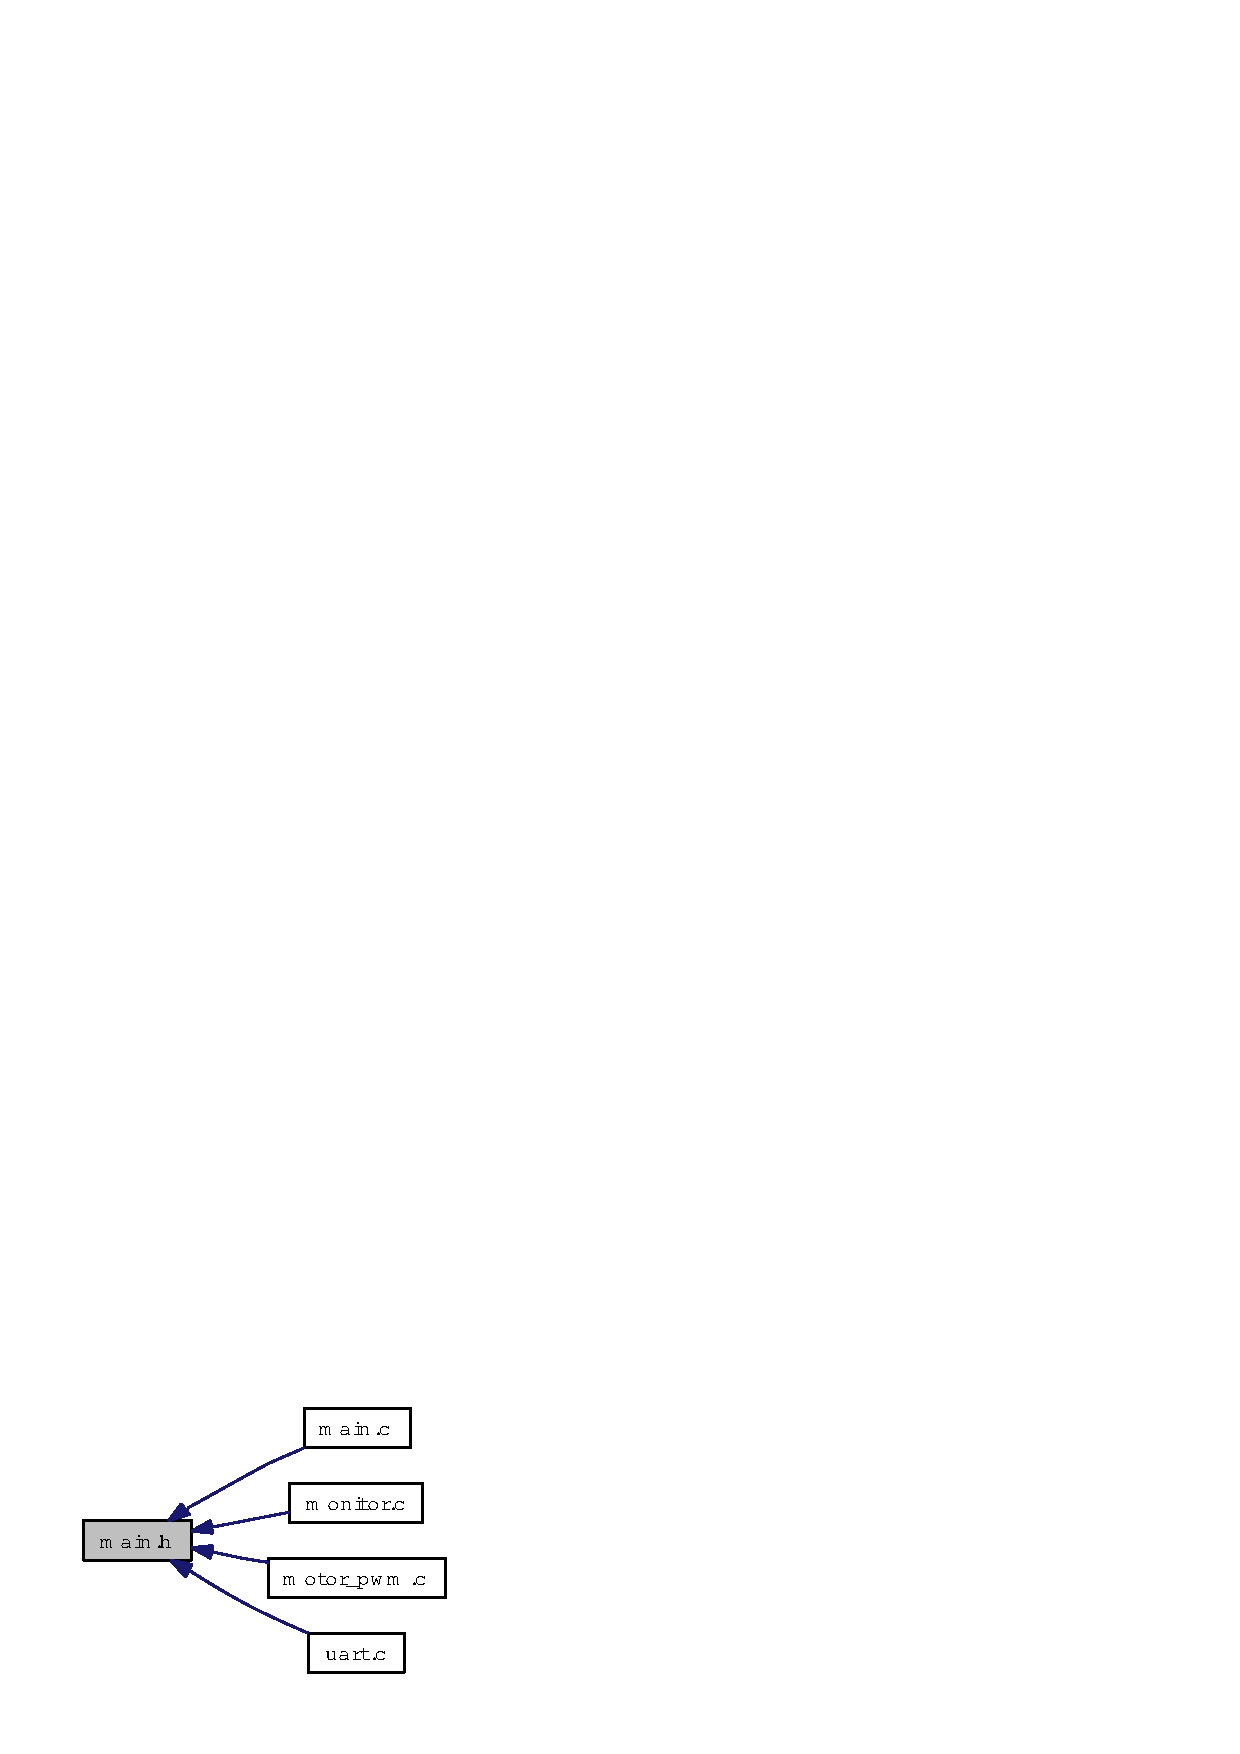
\includegraphics[width=109pt]{main_8h__dep__incl}
\end{center}
\end{figure}
\begin{CompactItemize}
\item 
\#define {\bf SYS\_\-CLK}~16000000
\item 
int {\bf main} (void)
\end{CompactItemize}


\subsection{Define Documentation}
\index{main.h@{main.h}!SYS_CLK@{SYS\_\-CLK}}
\index{SYS_CLK@{SYS\_\-CLK}!main.h@{main.h}}
\subsubsection{\setlength{\rightskip}{0pt plus 5cm}\#define SYS\_\-CLK~16000000}\label{main_8h_b3a7892b9f9fbb5c3fc2cbdbceb10017}




Definition at line 36 of file main.h.

Referenced by monitor(), and set\_\-motor\_\-pwm\_\-freq().

\subsection{Function Documentation}
\index{main.h@{main.h}!main@{main}}
\index{main@{main}!main.h@{main.h}}
\subsubsection{\setlength{\rightskip}{0pt plus 5cm}int main (void)}\label{main_8h_840291bc02cba5474a4cb46a9b9566fe}




Definition at line 163 of file main.c.

References disable\_\-motor1(), disable\_\-motor2(), init\_\-accel\_\-capture(), init\_\-adc(), init\_\-irled\_\-pwm(), init\_\-motor\_\-pwm(), init\_\-port\_\-directions(), init\_\-port\_\-values(), init\_\-uart(), MC13192\_\-init(), print\_\-status(), set\_\-led(), set\_\-motor1(), set\_\-motor2(), set\_\-motor\_\-pwm\_\-freq(), and uart\_\-puts\_\-P.

Here is the call graph for this function:\begin{figure}[H]
\begin{center}
\leavevmode
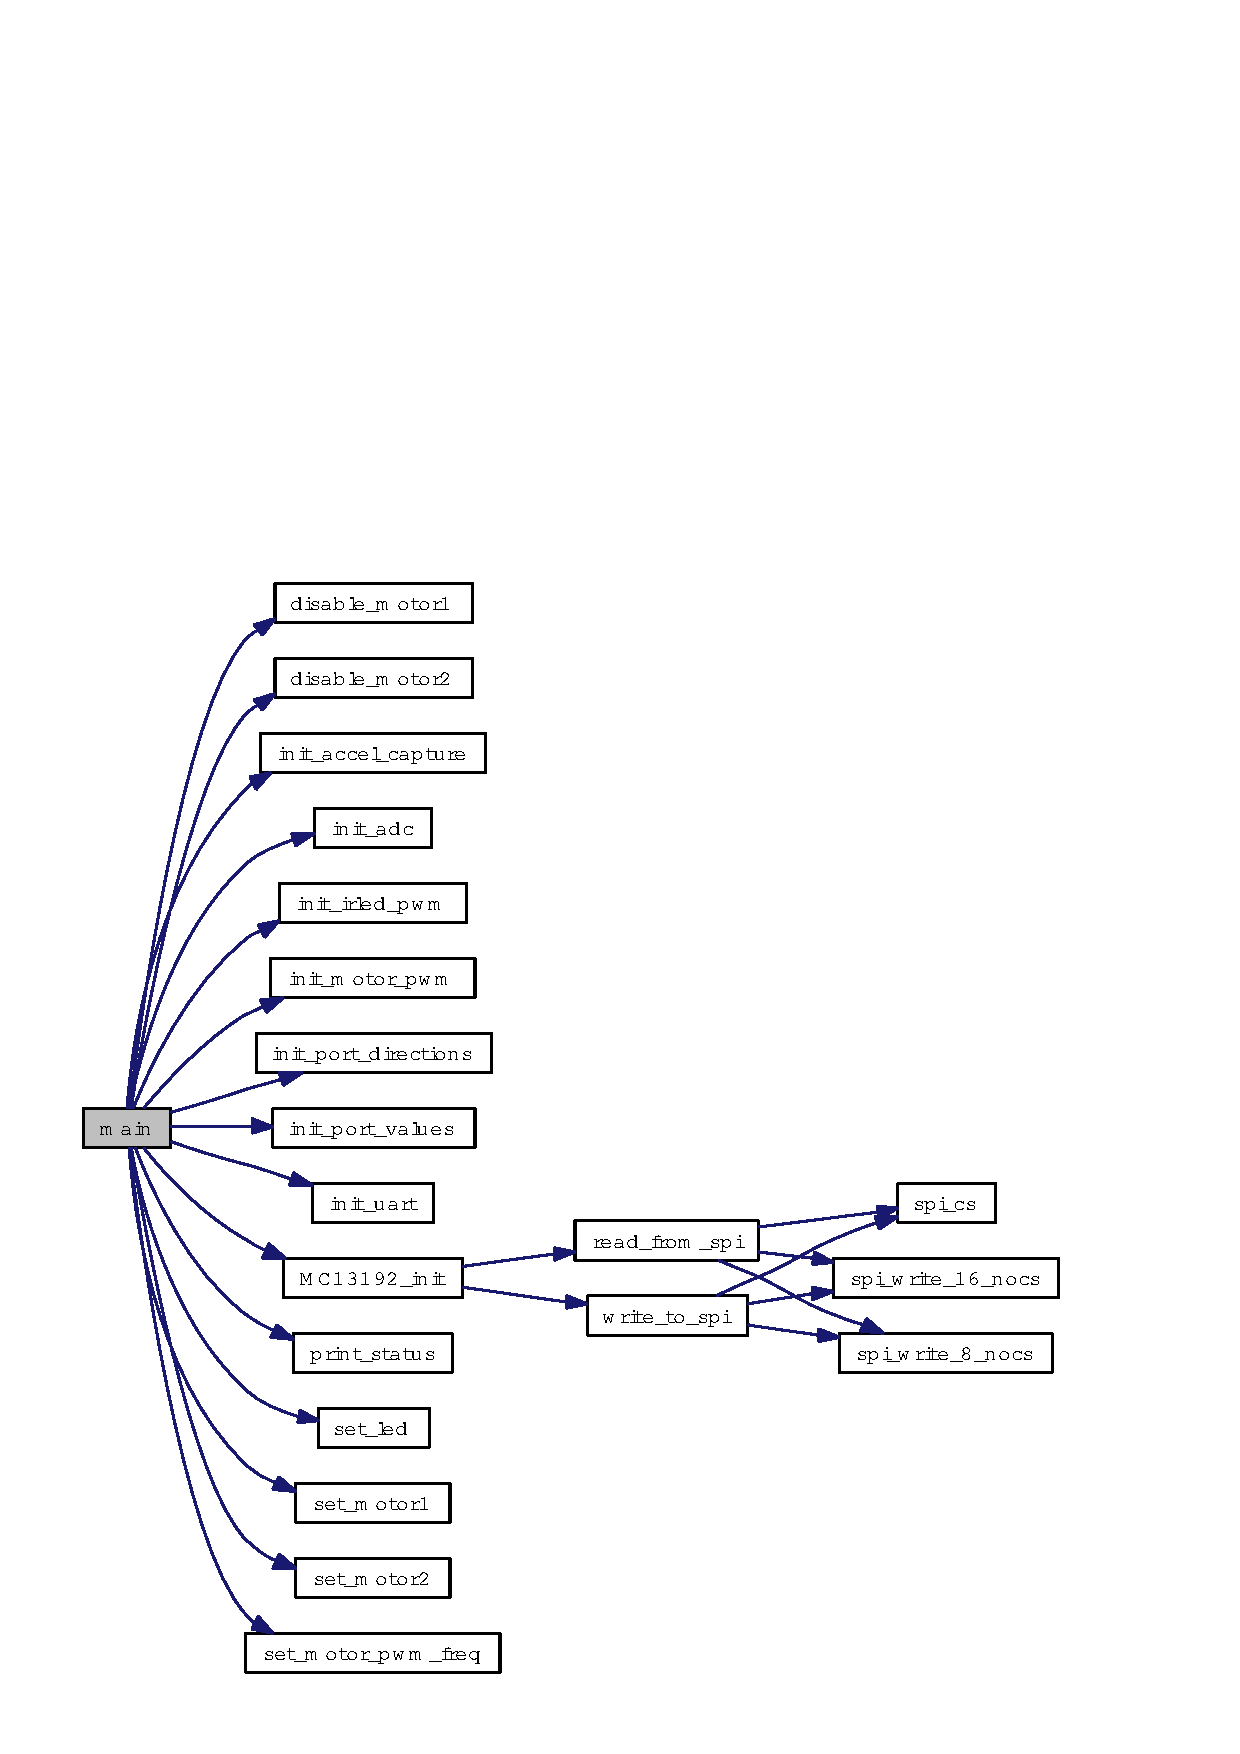
\includegraphics[width=256pt]{main_8h_840291bc02cba5474a4cb46a9b9566fe_cgraph}
\end{center}
\end{figure}
